\chapter{Caratteristica I-V di una lampadina}

\renewcommand\thesection{\Roman{section}}

\section{Resistenze interne di due tester}
\textbf{Obiettivo:} ricavare la resistenza interna di un tester digitale e di un tester analogico.

\paragraph{Strumentazione:}
\begin{enumerate}
    \item un alimentatore di tensione continua;
    \item una resistenza di $\SI{470}{\kilo\Omega}\pm5\%$;
    \item un tester digitale e un tester analogico.
\end{enumerate}

\paragraph{Procedura:}
\begin{enumerate}
    \item accendere il generatore di tensione e cortocircuitarlo impostando la corrente massima erogabile dal generatore a $\SI{0.1}{A}$;
    \item spegnere il generatore e impostare il tester digitale su volt. Per il tester analogico, impostarlo sul fondo scala $\SI{10}{V}$;
    \item Costruire sulla basetta di plexiglas il circuito;
    \begin{figure}[h]
        \centering
        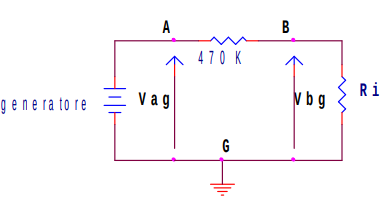
\includegraphics[width=0.5\linewidth]{Immagini/EXP1 - circuito strumenti misura.png}
        \caption{circuito per la misura  delle resistenze interne.}
        \label{fig: EXP1 - circuito strumenti misura}
    \end{figure}
    \item prima di dare tensione ricordare che il tester analogico di cui si dispone non ha protezioni quindi una manovra errata può portare al danneggiamento del tester.
    \item accendere l'alimentatore e regolarlo su circa $\SI{8}{V}$, leggere la tensione $V_{bg}$ con il tester
    \item scollegare il tester e misurare la tensione $V_{ag}$ con il tester.
    \item determinare la resistenza interna $R_i$ corredata della sua incertezza con
    \begin{equation}
        \frac{V_{ag}R_i}{470\times10^3+R_i}=V_{bg};
    \end{equation}
    \item ripetere la misura usando il tester digitale.
\end{enumerate}

\section{Caratteristica I-V di una lampadina}

\paragraph{Obiettivo:} ricavare la caratteristica I-V di una lampadina e verificare la validità della legge di corpo nero per un filamento di tungsteno riscaldato.

\paragraph{Strumentazione:}
\begin{enumerate}
    \item un alimentatore di tensione continua;
    \item una lampadina ad incandescenza;
    \item un tester digitale da usare come voltmetro e un altro da usare come amperometro.
\end{enumerate}

\paragraph{Procedura:}
\begin{enumerate}
    \item misurare la resistenza della lampadina a freddo;
    \item costruire il circuito;
    \begin{figure}[h]
        \centering
        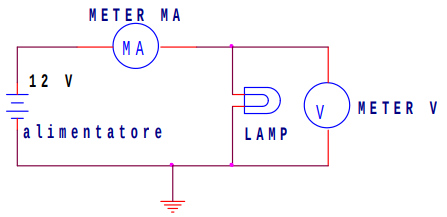
\includegraphics[width=0.6\linewidth]{Immagini/EXP1 - IV lampadina.png}
        \caption{circuito per la I-V della lampadina.}
        \label{fig:EXP1 - IV lampadina}
    \end{figure}
    \item variare il valore di tensione $V_{in}$ fornito dal generatore, da 0 V a 12 V, a passi di 0.5 V. Per ogni valore di tensione $V_{in}$, effettuare una misura di corrente e di tensione ai capi della lampadina. Si devono effettuare tutte le misure in una volta, in progressione ordinata;
    \item ricavare la resistenza della lampadina e la potenza dissipata;
    \item disegnare le funzioni $I(V)$, $R(V)$ e $P(R)$ ed effettuare una regressione sulle ultime due per determinare il valore di $q$; 
    \item i modelli da provare per le regressioni sono $f=aR^4$, $f=a(R^4-b^4)$ e $f=k(T-T_0)+c(T^4-T_0^4)$;
    \item determinare il range di validità di ogni modello.
\end{enumerate}

\setcounter{section}{0}
\renewcommand\thesection{\Alph{section}}

\section{Parametrizzazione \texorpdfstring{$I(V)$}{I(V)}}
Per alcuni materiali, come il tungsteno (metallo di transizione), una buona
rappresentazione dei dati sperimentali si ottiene invece con la relazione
\begin{equation}
    R=R_0\left(\frac{T}{T_0}\right)^b\quad\therefore\quad T=\beta R^{\gamma}.
\end{equation}
Più $\gamma$ è diverso dal valore unitario, meno la relazione tra T ed R si può approssimare da una proporzionalità diretta.

La lampadina consuma la potenza $P=VI$, dissipata in una piccola parte per via
conduttiva e convettiva, $k(T-T_0)$, e per la maggior parte per via radiativa, secondo la legge di corpo nero $P=e\sigma A_s(T^4-T_0^4)$. In prima approssimazione si può trascurare $T_0$ in quanto $T_{filamento}\approx\SI{2000}{\celsius}$. Quindi si ha
\begin{equation}
    P=VI=cT^4=c(\beta R^{\gamma})^4=mR^q,\quad q=4\gamma.
\end{equation}
Ricordando che $R=V/I$ si trova
\begin{equation}
    I=\sqrt[q+1]{m}V^{\frac{q-1}{q+1}}=sV^{\frac{q-1}{q+1}}.
\end{equation}